% در این بخش استانداردهای را تدوین خواهیم کرد که بر اساس آنها مستند نوشته می‌شود
% با این کار نه تنها می‌توانیم استانداردهای مناسبی را برای مستند نویسی ایجاد
% کنیم بلکه استانداردهای ایجاد شده را به مرور زمان به دیگران انتقال دهیم.

\chapter{چطور و کجا}

معمولا توسعه دهندگان سیستم‌های نرم‌افزاری، برای مستند کردن برنامه‌های نوشته شده
پروژه را بازبینی نخواهند کرد، از این رو توصیه می‌شود هر زمان که قسمتی از برنامه ایجاد و یا تغییر کرد
مستند آن نیز به صورت کامل نوشته شود. به ویژه از این میان مستند پیاده‌سازی از اهمیت بیشتری
برخوردار است چرا که گذر زمان منجر به فراموشی روش‌های مورد استفاده توسط
توسعه‌‌گر سیستم خواهد شد. معمولا در توسعه یک نرم‌افزار، هر بخش به صورت
مستقل نیاز به پیاده‌سازی، تست، و مستند سازی دارد. مهم نیست که این کارها به چه
ترتیبی اجرا می‌شوند اما به یاد داشته باشید که تمام آنها باید به صورت کامل انجام
شود.

  مستند فنی و پیاده‌سازی تنها مستندهایی هستند که در خود متن برنامه نوشته
  می‌شونداما در این مستندها تنها به توضیح و شرح کلاسها متدهای و ساختار برنامه
  پرداخته نمی‌شود. علاوه بر مستند برنامه‌های نوشته شده،
  اطلاعات جانبی دیگر مانند روش نصب، پیش نیازها، توانایی‌های جدید در برنامه و
  غیره نیز باید در مستند تکنیکی ایجاد شود. هدف اصلی این گفتار
  تعیین یک چهار چوب مناسب برای نوشتن تمام اطلاعات مورد نیاز در یک مستند تکنیکی
  است. در ادامه پس  از یک مرور کوتاه بر بخش‌های متفاوت یک مستند تکنیکی، در
  بخشهای جداگانه به صورت جزئی هر یک تشریح خواهد شد.

  ابتدایی ترین نیاز در یک مستند تکنیکی، تنظیماتی است که بر اساس آن یک
  مستند تکنیکی ایجاد می‌شود مانند نام پروژه تاریخ ایجاد، شماره نسخه و مسیر متن
  برنامه. برای تعیین این خصوصیت‌ها در مسیر اصلی پروژه یک پرونده به نام
  \lr{Doxygen} ایجاد می‌شود که همان پرونده پیکره بندی مستند است. این پرونده را
  می‌توان با استفاده از ویرایشگر \lr{Doxygen} و یا به صورت دستی ویرایش و
  تمام اطلاعات اصلی مورد نیاز برای ایجاد مستند را در آن ایجاد کرد.

  علاوه بر پرونده پیکره بندی یک پرونده به نام \lr{main.doxy} ایجاد می‌شود که
  توضیحات کلی در مورد پروژه در این پرونده نوشته می‌شود. همانگونه که در زبانهای
  برنامه سازی یک متد و یا فراخوانی به عنوان آغاز برنامه در نظر گرفته می‌شود در
  اینجا نیز این پرونده به عنوان نقطه آغاز مستند فنی در نظر گرفته می‌شود. مستند
  نوشته شده در این پرونده بر اساس استانداردهایی است که در ابزار تولید مستند
  \lr{Doxygen} تعیین شده است.

  همواره مستندهایی که در رابطه با متن اصلی برنامه نیست در پرونده‌هایی با پسوند
  \lr{*.doxy} ذخیره می‌شود. برای نمونه پرونده \lr{main.doxy} که در برگیرنده
  اطلاعات کلی از پروژه است نیز به صورت یک پرونده با همین پسوند ایجاد
  می‌شود. این نوع نام گذاری منجر به خوانایی مستند خواهد شده.

  تمام اطلاعات جانبی ایجاد شده در مورد یک پروژه، برای جلوگیری از به هم ریختگی،
  در یک پوشه به نام \lr{doc} نگه داری می‌شوند. تمام پرونده‌های ایجاد شده در این
  مسیر باید با پسوند \lr{*.doxy} بوده و بر اساس استاداردهای تعیین شده در
  \lr{Doxygen} ایجاد شده باشند. \lr{main.doxy} تنها پرونده‌ای است که در این مسیر
  قرار نمی‌گیرد.
  
  مستندهای مهم دیگر مانند روش ترجمه، نصب و راه اندازی پروژه هستند که به عنوان 
مستندهای اساسی هر پروژه‌ای در نظر گرفته می‌شوند. این مستند ها در
  یک پرونده به نام \lr{install.doxy} و در مسیر \lr{doc} نوشته می‌شوند.
 این مستند باید به صورت کامل و بر
  اساس سکوهای متفاوت روش نصب را تشریح کرده باشد. علاوه بر روش نصب و ترجمه باید
  پیش نیازهای سیستم و سکوهای مورد حمایت به صورت کامل و با
  جزئیات تشریح شده باشد. علاوه بر چگونگی نصب و راه اندازه یک بسته نرم افزاری
  مستندهایی در باب مبانی به کار رفته در نرم افزار، کاربردها، خطاها و پرسشهای
  متداول نیز مورد نیاز است و باید به مستند اضافه شود. با استفاده از این مستندها
  خواننده می‌تواند به سادگی به اطلاعات مورد نیاز را کسب کند، خطاهای متداول را بشناسد
  و بر اساس مبانی  سیستم را به کار ببندد.
  
  ساده ترین روش برای ساختاردهای کردن و دسته بندی کردن مستند استفاده از
  پیمانه‌ها یا \lr{Module}ها است. ابتدایی‌ترین روش ایجاد پیمانه‌ها در مکانهایی است
  که از آنها استفاده می‌شود. ایجاد پیمانه‌ها در هر مکان منجر به یک از هم
  گسیختگی در ایجاد و مدیریت پیمانه‌ها می‌شود تا جایی که ممکن است یک پیمانه با
  شناسه خاص در چند مکان و با کاربردهای متفاوت مورد استفاده قرار گیرد. این حالت
  زمانی که اندازه پروژه و تعداد توسعه دهندگان آن زیاد باشد به یک مشکل اساسی
  مبدل خواهد شد. از این رو در مسیر \lr{doc} یک پرونده به نام \lr{module} ایجاد
  می‌شود و تمام پیمانه‌های مورد نیاز به صورت جداگانه در آن تعریف می شود. پرونده
  ایجاد شده هر پیمانه با شناسه آن پیمانه نام گذاری می‌شود تا به راحتی بتوان با دیدن نام پرونده از
  شناسه آن اگاهی یافت. البته باید شناسه هر پیمانه نیز به گونه‌ای تعیین
  شده باشد که نه تنها بیانگر مطالب آن پیمانه باشد بلکه بر اساس قواعد نام‌گذاری 
پیمانه‌ها در \lr{Doxygen} تعیین شده باشد. با این
  روش تمام توسعه دهندگان سیستم و حتی افرادی که عضو گروه توسعه نیستند
  می‌توانند به سادگی از تمام مستندهای ایجاد شده و ساختار آنها آگاهی پیدا کنند.
  
  در بسیاری از مستندهای تکنیکی از چندین نمونه برای تشریح کامل سیستم استفاده
  می‌شود. به ویژه زمانی که سیستم یک بسته نرم‌افزاری است و به عنوان یک قطعه در
  دیگر پروژه‌ها مورد استفاده قرار می‌گیرد.برای ایجاد نمونه‌ها در مسیر \lr{doc}
  یک پوشه جدید به نام \lr{tutorial} ایجاد می‌شود و نمونه‌ها به صورت جداگانه در
  این مسیر ایجاد می‌شوند. یک پوشه دیگر نیز با نام \lr{image} ساخته می‌شود و تمام 
  تصاویر مورد استفاده در متن مستند در آن پوشه قرار می‌گیرد.
  
  در تصویر شماره \ref{standard/where-what/doc-struct} ساختار کلی یک پروژه نمونه آمده است.
  همانگونه که در این تصویر قابل مشاهد است، پرونده‌ها و پوشه‌های متفاوتی در یک
  پروژه ایجاد می‌شود تا بتوان یک مستند مناسب تکنیکی را به وجود آورد. گرچه این
  ساختار بر اساس تجربه‌های متفاوت در نوشتن مستندهای تکنیکی تکمیل شده است اما
  می‌توان آن را بر اساس نیازهای یک پروژه به روز کرد. در ادامه این گفتار هرکدام
  موارد مطرح شه به صورت کامل تشریح خواهد شد.
%   FIXME :هادی ۱۳۹۱ :تصویر بر اساس ساختار توضیح داده شده اصلاح شود.
  \begin{figure}
    \centering
    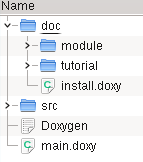
\includegraphics[width=0.4\textwidth]{image/doc-struct}
    \caption[ساختار مورد نیاز برای ایجاد مستند تکنیکی]
    {
      ساختار مورد نیاز برای یک مستند تکنیکی. هماگونه که در این تصویر قابل مشاهده
      است یک مسیر به نام \lr{doc} ایجاد می‌شود و مستندهای جانبی در آن قرار
      می‌گیرد. دیگر مستندها در متن برنامه نوشته می‌شود.
    }
    \label{standard/where-what/doc-struct}
  \end{figure}


%
% حق نشر 1390-1402 دانش پژوهان ققنوس
% حقوق این اثر محفوظ است.
% 
% استفاده مجدد از متن و یا نتایج این اثر در هر شکل غیر قانونی است مگر اینکه متن حق
% نشر بالا در ابتدای تمامی مستندهای و یا برنامه‌های به دست آمده از این اثر
% بازنویسی شود. این کار باید برای تمامی مستندها، متنهای تبلیغاتی برنامه‌های
% کاربردی و سایر مواردی که از این اثر به دست می‌آید مندرج شده و در قسمت تقدیر از
% صاحب این اثر نام برده شود.
% 
% نام گروه دانش پژوهان ققنوس ممکن است در محصولات دست آمده شده از این اثر درج
% نشود که در این حالت با مطالبی که در بالا اورده شده در تضاد نیست. برای اطلاع
% بیشتر در مورد حق نشر آدرس زیر مراجعه کنید:
% 
% http://dpq.co.ir/licence
%
\section{پیکره بندی}
در این قسمت به بررسی پرونده پیکر بندی مورد نیاز برای ایجاد مستن خواهیم پرداخت
در این پرونده علاوه بر این که تنظیمات اولیه مورد نیاز برای ایجاد مستند وجود
دارد چگونگی ایجاد مستند نیز به صورت کامل تشریح می‌شود. همواره فرض می‌شود که هر
پروژه یا قطعه در یک پروژه به صورت کامل در یک پوشه هم نام با آن قرار دارد. تمام
قطعه‌ها و پروژه‌هایی که با هم دیگر یک پروژه کلی را ایجاد می‌کنند نیز کنار یک
دیگر و در یک پوشه قرار می‌گیرند.

مستند تکنیکی ایجاد شده از سیستم نیز خود یک زیر پروژه از پروژه کلی در نظر گرفته
می‌شود از این رو باید یک پوشه، در پوشه پروژه اصلی در نظر گرفت. این پوشه را
همواره با نام \lr{doc} در نظر می‌گیریم. مستند تکنیکی هر زیر پروژه باید به صورت
یک پرونده هم نام با همان زیر پروژه در پوشه \lr{doc} ایجاد شود. برای نمونه فرض
کنید که در پروژه اصلی سه زیر پروژه به نام‌های \lr{GUI}، \lr{Shell} و \lr{LIB}
وجود دارد. در این صورت در این پروژه یک پوشه دیگر به نام \lr{doc} باید ایجاد
و معادل با هر زیر پروژه در آن یک پوشه ایجاد شود. در شکل
\ref{wher-what-config-example-1} ساختار مورد نیاز برای این پروژه نمایش داده
شده است.

در گام بعد در هر پروژه یک پرونده پیکره بندی برای مستند فنی به نام \lr{Doxygen}
ایجاد می‌شود که داده‌های مورد نیاز برای ایجاد مستند در آن قرار خواهد گرفت. در
شکل \ref{wher-what-config-example-1} محل قرار گرفتن پرونده‌های پیکره بندی نشان
داده شده است. از آنجا که محل خروجی مستندهای ایجاد شده بر اساس تنظیم‌های موجود
در همین پرونده‌های تعیین می‌شود باید خصوصیت مسیر خروجی برای هر مستند را به
گونه‌ای اصلاح کرد که مستندهای ایجاد شده در مسیر مناسب قرار گیرد. برای نمون در
پرونده پیکربندی پروژه \lr{GUI} مسیر خروجی به صورت زیر اصلاح می‌شود:

\begin{latin}
\lstset{language=bash}  
\begin{lstlisting}[frame=single] 
OUTPUT_DIRECTORY       = ../doc/GUI
INPUT                  = ./
\end{lstlisting}
\end{latin}

همانگونه که در نمونه آورده شده قابل مشاهده است علاوه بر مسیر خروجی باید مسیر
ورودی پروژه را نیز تعیین کرد. از آنجا که برای هر پروژه به صورت جداگانه یک پرونده
پیکره بندی ایجاد می‌شود کافی است که مسیر ورودی را مسیر جاری قرار داد. با این
تنظیم بدون ترس از محل قرار گرفتن مستند‌ها می‌توان به سادگی در پایان پروژه مستند
فنی را بر اساس تمام پروژه‌ها موجود در پروژه اصلی ایجاد کرد. این فرآیند می‌تواند
به صورت خودکار در پروژه‌های بزرگ انجام شود.

مستندگر \lr{Doxygen} تنها مسیر ورودی تعیین شده را برای یافتن پرونده‌های ورودی
جستجو می‌کند، در صورتی که ساختار تشریح شده برای مستندها و برنامه‌ها به صورت
سلسله مراتبی در نظر گرفته شده است. در این حالت در پرونده پیکره بندی باید جستجوی
بازگشتی برای یافتن پرونده‌ها فعال شود. برای فعال کردن این روش جستجو باید تنظیم
زیر را در پرونده پیکره بندی اضافه کرد:

\begin{latin}
\lstset{language=bash}  
\begin{lstlisting}[frame=single] 
FILE_PATTERNS          = *.h \
                         *.hh \
                         *.hxx \
                         *.hpp \
                         *.h++ \
                         *.dox \
                         *.doxy

RECURSIVE              = YES
\end{lstlisting}
\end{latin}

همانگونه که در کده بالا قابل مشاهده است علاوه بر فعال کردن جستجوی بازگشتی،
می‌بایست ساختارها و پرونده‌هایی که باید به عنوان ورودی قرار گیرد را تعیین کرد.
گرچه که پرونده‌های ورودی وابسته بر اساس نوع پروژه و زبان‌های برنامه سازی به کار
گرفته شده در آن تعیین می‌شود، اما در هر حال پرونده‌های با پسونده \lr{*.doxy}
باید همواره به عنوان ورودی مورد استفاده قرار گیرد.

علاوه بر تمام خصوصیت‌هایی که در این بخش مورد بررسی قرار گرفت خصوصیت‌های دیگری
نیز وجود دارد که باید در یک پرونده پیکرده بندی تعیین شوند. در کد زیر  برخی از
مهم‌ترین تنظیم‌های مورد نیاز برای یک پروزه آورده شده است:

\begin{latin}
\lstset{language=bash}  
\begin{lstlisting}[frame=single] 
DOXYFILE_ENCODING      = UTF-8
PROJECT_NAME           = My Project GUI
PROJECT_NUMBER         = 0.1.0 beta
PROJECT_BRIEF          = MGUI
PROJECT_LOGO           = ./images/logo.png
\end{lstlisting}
\end{latin}

در نهایت با ایجاد تنظیم‌های مورد نیاز برای تمام پروژه‌ها می‌توان به سادگی مستند
فنی مورد نیاز برای پروژه را ایجاد و در موقع نیاز از آنها استفاده کرد.

%
% حق نشر 1390-1402 دانش پژوهان ققنوس
% حقوق این اثر محفوظ است.
% 
% استفاده مجدد از متن و یا نتایج این اثر در هر شکل غیر قانونی است مگر اینکه متن حق
% نشر بالا در ابتدای تمامی مستندهای و یا برنامه‌های به دست آمده از این اثر
% بازنویسی شود. این کار باید برای تمامی مستندها، متنهای تبلیغاتی برنامه‌های
% کاربردی و سایر مواردی که از این اثر به دست می‌آید مندرج شده و در قسمت تقدیر از
% صاحب این اثر نام برده شود.
% 
% نام گروه دانش پژوهان ققنوس ممکن است در محصولات دست آمده شده از این اثر درج
% نشود که در این حالت با مطالبی که در بالا اورده شده در تضاد نیست. برای اطلاع
% بیشتر در مورد حق نشر آدرس زیر مراجعه کنید:
% 
% http://dpq.co.ir/licence
%
\section{برگه نخست}
  برگه نخست ابتدایی ترین قسمت در یک مستند است، از این جهت در ایجاد و سازمان دهی
  یک مستند بسیار مهم است.
  اگر این صفحه به درستی و به شیوه مناسب طراحی و ایجاد نشده باشد، خواننده مستند
  نمی‌تواند به سادگی مستند را مور استفاده قرار دهد و در نخستین برخورد دچاد
  سردرگمی خواهد شد.

  پیش از هر چیز باید به این نکته اشاره کرد که برگه عبارت است از یک بخش از مستند
  که در حالت کلی معادل با یک گفتار در یک کتاب است.
  هر برگه را در یک پرونده \lr{*.doxy} ایجاد می‌شود و در آن متن برگه به صورت کامل
  نوشته می‌شود.
  هر برگه همانند یک گفتار می‌تواند از بخشهای متفاوتی ایجاد شده باشد.
  هر بخش و زیر بخشهای آن نیز به صورت منظم و پشت سرم هم در پرونده برگه نوشته
  می‌شود. در کد زیر نمونه‌ای از یک برگه آورده شده است.
  
\begin{latin}
\lstset{language=C++}
\begin{lstlisting}[frame=single] 
/**
\page pageid Page Title
  Page Body.
  
  \section sectionid Section Title
    Section Body.

    \subsection subsectionid Subsection Title
      Subsection Body.
*/
\end{lstlisting}
\end{latin}

  همانگونه گه پیش از این نیز گفته شد، برگه نخست ابتدایی ترین قسمتی از مستند است
  که هر خواننده با آن روبرو می‌شود. بی شک انتخاب دقیق مطالب مورد نیاز و
  ساختاردهی آن در تاثیر پذیری آن اثر خواهد داشت.
  در نخستین قسمت از برگه نخست باید به معرفی نرم افزار و بیان اهداف اصلی طراحی و
  ایجاد آن اختصاص داده شود.
  هر خواننده با دانستن اهداف یک نرم‌افزار یا بسته نرم‌افزاری می‌تواند به چرایی
  بسیاری از رویکردهای سیستم پاسخ دهد.
  دور از ذهن نیست که برای انجام هر پردازش ویا اجرای هر فرآیند در یک سیستم
  نرم‌افزاری روش‌های متفاوتی وجود داشته باشد. برای نمونه در ذخیره و بازیابی
  داده‌های می‌توان از روش‌های متفاوتی چو پایگاه داده‌ها، پرونده‌های متنی و
  باینری و یا بسیاری از روش‌های دیگر استفاده کرد. واضح است که خواننده با اشراف
  بر اهداف یک سیستم می‌تواند به راحتی درک کند که چرا در یک مسئله از روشی خاص
  استفاده شده است و در نتیجه توانایی و محدودیت سیستم در کجا است.

  در توسعه یک سیستم مدیران پروژه در نخستین گام به دنبال سیستم‌های موجودی خواهند
  بود که بتواند تمام اهداف مورد نظر آنها را پوشش دهد. در بسیاری از موارد نیز
  اهداف و نیازهای سیستم مورد بازبینی قرار گرفته و گه گاه از آنها کاسته می‌شود تا
  کاملا با اهداف یک سیستم موجود هم سو شود. در این صورت ابتدایی ترین پرسش مطرح
  برای یک مدیر اهداف یک سیستم ایجاد شده است. بر این اساس ایجاد یک بخش مجزا و
  تشریح اهداف یک سیستم بسیار اساسی به نظر می‌رسد.

  شکی نیست که پیش از هرچیز در یک مستند تکنیکی باید سیستم را به صورت کامل تعریف
  کرد و اهداف مورد نظر در طراحی و پیاده سازی آن را تشریح کرد اما علاوه بر این
  نیاز است که ساختار مستند نیز به صورت کامل تشریح شود. این تصور اشتبا است که
  همواره هر خواننده از ابتدایی ترین موضوع در مستند شروع کرده و تا انتها تمام
  ستند را به ترتیب مطالعه خواهد کرد.
  خوانندگان یک مستند با دیدگاهی متفاوت تنها به دنبال دسته‌ای خاص از اطلاعات
  ایجاد شده در یک مستند هستند و از خواندن بسیار از بخشهای مستند صرف نظر خواهند
  کرد. در این حالت معرفی مفید و کامل ساختار مستند می‌تواند بسیار مفید واقع شود و
  احساس خوبی را در خوانندگانی که برای اولین بار مستند را مطالعه می‌کنند ایجاد
  کند.

  مدیران  سیستم‌های نرم افزاری در فرآیند گزینش یک سیستم جدید در پی داده‌های چون
  سخت‌افزارهای مورد نیاز، وابستگی به بسته‌های نرم‌افزاری دیگر، قابلیت انتقال به
  روی سکوی‌های متفاوت و دیگر اطلاعات از یک سیستم موجود هستند. این در حالی است که
  توسعه دهندگان سیستم‌های نرم افزاری بیشت به دنبال اطلاعاتی در زمینه به کار گیری
  سیستم در کاربردهای مورد نظر هستند. اینها تنها بخشی از خوانندگان با دیدهای
  متفاوت هستند که مستند تکنیکی سیستم‌های موجود را مورد بررسی و مطالعه قرار
  می‌دهد. در چنین شرایطی ایجاد ساختار مناسب در مستندها و تشریح کافی و کامل آن
  می‌تواند خوانندگان را در یافتن اطلاعات مورد نظرشان از یک سیستم موجود یاری کند.

  سومین بخش از برگه نخست مستند که باید در نظر گرفته شود، بیان سطوح متفاوت موجود
  در یک مستند و توصیه‌های مناسب برای خوانندگان مستند است. بی شک مستند یک سیستم،
  به خصوص زمانی که اندازه سیستم بزرگ است، زمینه‌های متفاوتی را پوشش داده و در
  نتیجه خوانندگان متفاوتی را به خود خواهد دید از این رو تعیین زمینه‌های متفاوت
  موجود و توصیه مناسب به خوانندگانی که قصد مطالعه مستند را دارند می‌تواند آنها
  را در یافتن مناسب اطلاعات مورد نیازشان یاری کند. در کد نمونه‌ای که در ادامه
  آورده شده است یک ساختار ابتدایی برای برگه نخست مستند ارائه شده است.
\begin{latin}
\lstset{language=C++}
\begin{lstlisting}[frame=single] 
/**
\mainpage
  Introduction

\section docstruct Document Structuer
  Document Struction

\subsection whoread Who Read
  Who Read

\section whatsnew New
  What is New

\section bugs Closed Bugs
  Bugs
*/
\end{lstlisting}
\end{latin}

  همان گونه که در متن مستند نوشته شده قابل مشاهد است، دو بخش جدید نیز در انتهای
  برگه نخست پیش بینی شده است.
  اولین بخش در مورد توانایی‌های جدیدی است که به نسخه جدید از سیستم اضافه شده است
  در حالی که دومین بخش در مورد خطا‌هایی است که از نسخه پیشین حذف شده است. این دو
  بخش در رابطه با سیستم‌هایی است که دورده زمانی زیادی را دارند و در نسخه‌های
  متفاوت توسعه می‌یابند.

  
%
% حق نشر 1390-1402 دانش پژوهان ققنوس
% حقوق این اثر محفوظ است.
% 
% استفاده مجدد از متن و یا نتایج این اثر در هر شکل غیر قانونی است مگر اینکه متن حق
% نشر بالا در ابتدای تمامی مستندهای و یا برنامه‌های به دست آمده از این اثر
% بازنویسی شود. این کار باید برای تمامی مستندها، متنهای تبلیغاتی برنامه‌های
% کاربردی و سایر مواردی که از این اثر به دست می‌آید مندرج شده و در قسمت تقدیر از
% صاحب این اثر نام برده شود.
% 
% نام گروه دانش پژوهان ققنوس ممکن است در محصولات دست آمده شده از این اثر درج
% نشود که در این حالت با مطالبی که در بالا اورده شده در تضاد نیست. برای اطلاع
% بیشتر در مورد حق نشر آدرس زیر مراجعه کنید:
% 
% http://dpq.co.ir/licence
%
\section{برگه‌های دیگر}
  علاوه بر برگه نخست برگه‌های دیگری نیز در مستند وجود دارند که جنبه‌های متفاوتی
  از سیستم را مورد بررسی قرار می‌دهند. نصب و راه اندازی، مبانی مورد استفاده در
  سیستم، به کارگیری و خطاهای متداول سیستم تنها بخشی از مستندهایی است که معمولا
  در یک مستند تکنیکی وجود دارد.

  به این نکته باید توجه داشت که در یک مستند تکنیکی دو جنبه کاملا مجزا و در عین حال
  تاثیر گذار وجود دارد: ساختار و سازماندهی مستندها. ساختار
  مستند (همانگونه که در بخش پیش به آن اشاره شد) به چینش و ترتیب مستندهای ظاهر
  شده در متن مستند گفته می‌شود. بخش‌ها زیر بخش‌ها گفتارها و جنبه‌هایی از سیستم که باید 
  مور بررسی قرار گیرد همگی موضوعاتی هستند که در ساختار دهی مستند مورد توجه قرار می‌گیرند.
 این درحالی است که سازمان
  دهی مستند فرآیندی است که در آن قرار دادن مستندها در مسیرهای مشخص، تعیین نام پرونده‌ها و مدیریت
  مستند ایجاد شده پرداخته می‌شود.

  برای نمونه این که تمام مستندهای جانبی باید در مسیر \lr{doc} قرار گیرد و با پسوند
  \lr{*.doxy} ذخیره شود به سازماندهی مستند است در حالی که معرفی سیستم و
  تشریح اهداف آن به ساختار مستند مربوط می‌شود.
  در طراحی مستند مناسب باید به هر دو جنبه مورد توجه باشد، از این رو در این بخش هر دو
  جنبه مورد بررسی قرار خواهد گرفت. از انجا که تعیین یک مرز کاملا مشخص بین این
  دو دشوار و در برخی موارد منجر به پیچیده شدن موضوع می‌شود هر دو آنها باهم مورد بررسی قرار خواهد گرفت.

  هر برگه معادل با یک فصل در نظر گرفته خواهد شد که در یک پرونده جدا با پشوند
  \lr{*.doxy} ایجاد می‌شود. از این رو برگه‌ها نیز باید در مسیر دیگر مستندهای
  جانبی یعنی در پوشه \lr{doc} قرار بگیرند.
  هر بخش با استفاده از برچسب \lr{page} در مستند مشخص شده که با استفاده از یک
  شناسه در کل مستند قابل آدرس دهی است.
  از آنجا که شناسه هر برگه منحصر به فرد است، استفاده از شناسه برگه به عنوان نام
  پرونده نه تنها مشکل نام گذاری پرونده‌ها را حل می‌کند بلکه منجر به دستیابی راحت
  به برگه‌ها در زمان توسعه مستند می‌شود. با این روش به سادگی و تنها با مشاهده
  نام پرونده می‌توان از مطالب درون آن اطلاع یافت.

  یک برگه می‌تواند به عنوان یک زیر بخش و یک زیر برگه از یک برگه دیگر در نظر
  گرفته شود (اضافه کردن یک برگه به عنوان زیربرگ در برگه دیگر با استفاده از برچسب
  \lr{subpage} انجام می‌شود که شرح کامل آن در بخش بسته بندی مستند آمده است).

  زمانی که تعداد زیربرگه‌های یک برگه زیاد می‌شود بهتر است که آنها را در یک پوشه
  جدا ( و هم نام با شناسه برگه) قرار داد. اما اگر تعداد زیر برگه‌ها کم باشد
  می‌توان آنها را در انتهای پرونده برگه اصلی اضافه کرد. مستند زیر یک نمونه از
  ایجاد برگه و زیر برگه‌ها در یک پرونده را نشان می‌دهد.

\begin{latin}
\lstset{language=C++}
\begin{lstlisting}[frame=single]
/**
\page pageid Example
  Page budy
  ....
  \subpage subpageid1
  \subpage subpageid2
  ....
*/
/**
\page subpageid1 Subpage Title 1
...
*/
....
\end{lstlisting}
\end{latin}

  مناسب ترین روش، ایجاد برگه‌های اصلی در مسیر \lr{doc} و ایجاد زیر برگه‌ها هر یک در زیر
  پوشه‌های مجزا به ازای هر برگه اصلی است - برگه اصلی در اینجا به معنی برگه‌هایی
  است که به عنوان زیر برگ هیچ برگ دیگر از مستند نباشد.

  تعیین برگه‌های اصلی مورد نیاز در هر مستند دشوار است و بسته به اندازه و نوع
  پروژه می‌تواند بسیار متفاوت باشد. اما دسته‌ای از این برگه‌ها
  تقریبا در تمام مستندهای تکنیکی وجود دارند.
  در فهرست زیر پر کاربرد ترین برگه‌های موجود در مستندهای تکنیکی آورده شده است:
  \begin{itemize}
   \item نصب و راه اندازی
   \item مبانی
   \item کاربردها
   \item پرسشهای متداول
  \end{itemize}
  در ادامه این بخش، این برگه‌ها به صورت مفصل‌تر مورد بررسی قرار  خواهد گرفت.

  
  
\subsection{نصب و راه اندازی}
  راهنمای نصب یک نرم‌افزار در بسیاری از موارد با راهنمای مدیریت و کاربری یک
  سیستم نرم افزاری و یا سخت افزاری هم پوشانی دارد. این هم پوشانی به دلیل وجود
  تنظیم‌های مورد نیاز در فرآیند نصب است که به عنوان حالت اولیه سیستم در نظر
  گرفته می‌شود.

  نصب و راه اندازی سیستم با تنظیم و به کارگیری آن در رابطه است و
  گاه شامل اطلاعاتی می‌شود که در مستندهای دیگر مانند مستند مدیریت و یا کاربری 
  هم پوشانی دارد. در این شرایط مناسب است که به مستندهای دیگر ارجاع داده شده و از
  ذکر دوباره اطلاعات خوداری کرد. اما باید به این نکته توجه داشت که بیان دوباره
  نکته‌های مهم می‌تواند در مستقل شدن مستند و نصب سریع و آسان سیستم کمک کند. به
  هر حال نباید از زیاده گویی و افزونگی مستند غافل شد.

  موارد متفاوتی وجود دارد که در این بخش باید به صورت کامل به آن پرداخته شود. در
  اینجا برخی از موارد لاز در فرآیند نصب و راه اندازی سیستم بیان و 
روش مستندسازی آنها مورد بررسی قرار گرفته شده است.


\paragraph{پیش نیازها}
   چه نوع نرم‌افزار، سخت افزار، و یا سکوی نرم‌افزاری برای نصب یک سیستم مورد نیاز
   است؟ آیا سیستم به روی هر سکوی نرم افزاری و یا سخت افزاری قابل اجرا است؟ آیا
   سیستم با سیستم‌های عامل متفاوت چون لینوکس، مک، و یا ویندوز سازگار است؟
   پردازشگر مورد نیاز سیستم چه قابلیت‌هایی باید داشته باشد؟ اینها بخشی از
   پرسش‌هایی است که باید در این بخش به آن پرداخته شود.

   توجه به این نکته بسیار مهم است که پیش‌نیازهای یک سیستم گاهی از خود آن نیز
   مهم‌تر می‌شود. برای نمونه حالتی را تصور کنید که در آن سیستم به صورتی ایجاد
   شده است که تنها به روی یک سیستم عامل خاص قابل اجرا است در این صورت فرد یا
   گروهی که به آن سیستم عامل دسترسی ندارند نمی‌توانند از این سیستم استفاده کنند.
   پیش‌نیازهای یک سیستم در انتخاب یک سیستم بسیار موثر خواهد بود.

   به عنوان نمونه در راهنمای نصب سیستم عامل ویندوز ویستا، موارد زیر به عنوان
   پیش‌نیاز نصب سیستم معرفی شده است:
\begin{config}
1 GHz 32-bit (x86) or 64-bit (x64) processor
512 MB of system memory
20 GB hard drive with at least 15 GB of available space
Support for DirectX 9 graphics and 32 MB of graphics memory
DVD-ROM drive
Audio Output
Internet access
\end{config}
   بر اساس این پیش‌نیازها کاربران و مدیران می‌توانند سیستم مورد نیاز
   خود را بر اساس پیش‌نیاز آنها انتخاب کنند. گرچه یک سیستم ایده آل سیستمی است که پیش‌نیازهای آن کم و
   با هر شرایطی سازگار باشد اما در هر حال باید پیش‌نیاز سیستم به درستی تعیین شده
   باشد تا کاربران در فرآیند نصب و راه اندازی سیستم با مشکل روبرو نشوند.
   
\paragraph{دست یابی به سیستم}
  پیش از هر کاری نیاز است که کاربران به نرم‌افزار و یا کد منبع آن دست پیدا کنند.
  در این بخش بر اساس توافق نامه یک نرم‌افزار به کاربران اطلات لازم جهت دست یابی
  که نرم افزار داده می‌شود. برای نمونه در سیستم های متن باز به کاربران آموزش
  داده می‌شود که چگونه با استفاده از مدیریت نسخه‌ها به یک نسخه خاص از کد منبع
  نرم‌افزار دست پیدا کنند.
  
\paragraph{تنظیم و نصب سریع}
   گاهی در مستند‌های فنی از این بخش به عنوان شروع سریع یاد می‌کنند که در آن
   فرآیند نصب و به کارگیری عملی سیستم با کمترین تنظیم و منابع تشریح می‌شود. به
   کارگیری ساده و سریع یک سیستم می‌تواند اعتماد کاربران را به سیستم افزایش دهد.

   در این بخش پیش شرط‌های مورد نیاز برای نصب، حالت نرم‌افزار و سخت‌افزارهای مورد
   استفاده و درک لازم از حالت سیستم به صورت کامل تشریح شده و کاربر برای نصب
   مقدماتی سیستم آماده می‌شود. علاوه بر این در این بخش عبارت‌ها و واژگان جدید
   مطرح در سیستم که حالت و یا قسمت خاصی از سیستم را تشریح می‌کند به صورت کامل
   بیان می‌شود.

   روش مناسب برای تعیین درک کامل از سیستم، تشریح سیستم و ساختار آن با
   استفاده از نمودارها است.
   ساختار سیستم، واسطه‌های مورد حمایت، شبکه‌های مورد استفاده و بسیاری دیگر از
   اجزای مورد نیاز سیستم را می‌توان با استفاده از یک نمودار به سادگی تشریح
   کرد و درک کاملی را از سیستم و پیش‌نیازهای آن به وجود آورد. درک سیستم نه تنها
   فرآیند نصب را قابل درک کرده بلکه کاربران را در تعیین و رفع مشکلات سیستم یاری
   می‌کند. در شکل 
   \ref{تصویر-ساختار-خوشه-پایگاه-داده}
    یک نمونه از شکل‌های مورد
   استفاده در راهنمای نصب یک سیستم نرم‌افزاری نمایش داده شده است.
  \begin{figure}
    \centering
    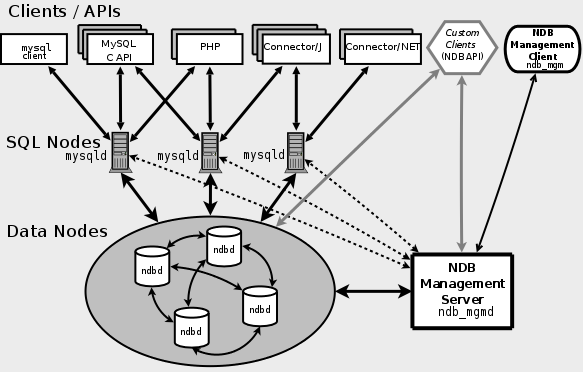
\includegraphics[width=0.75\textwidth]{image/mysql-cluster-install.png}
    \caption[ساختار خوشه‌ای پایگاه داده]
    {
      در این تصویر ساختار خوشه‌ای \lr{MySQL} نمایش داده شده است. بر اساس این
      ساختار کاربران می‌توانند پیش نیازهای سیستم را در نصب خوشه‌ای و تفاوت آن را
      با دیگر روش‌های نصب در این نرم افزار درک کند.
      از این شکل در راهنمای نصب این نرم‌افزار استفاده شده است.
    }
    \label{تصویر-ساختار-خوشه-پایگاه-داده}
  \end{figure}
  
   کاربران سیستم در اولین برخورد و مبتنی بر مستندهای این بخش است که قادر خواهند بود
   سیستم را به صورت عملی نصب کرده و به کار ببرند. لذا طراحی و نوشتن مناسب این بخش
   می‌تواند در جلب اعتماد کاربران بسیار مفید باشد. به این نکته توجه داشته باشید
   که زمانی یک کاربر به سیستم اعتماد کند آن را به کار خواهد بست و در ادامه
   تنظیم‌های پیشرفته سیستم را نیز فرا خواهد گرفت. پژوهشها نشان می‌دهد که عدم
   توانایی نصب راحت و به کار گیری یک سیستم منجر به کاهش علاقه کاربران در به
   کارگیری سیستم خواهد شد از این رو پرداختن به این بخش می‌تواند بسیار مهم باشد.

\paragraph{آزمون و خطایابی}
    تمام سیستم‌های نرم‌افزاری و سخت‌افزاری از روش‌های متفاوتی برای نمایش حالت
    درونی سیستم استفاده می‌کنند.
    واسطه‌ها گرافیکی، پیام‌های صوتی تصویری، دریچه‌های محاوره‌ای بخشی از روکردهای
    مورد استفاده در نمایش حالت درونی یک سیستم نرم‌افزاری است. سیستم‌های
    نرم‌افزاری با استفاده از همین رویکردها رویدادهای داخلی سیستم را به
    کاربران گزارش می‌کنند.

    در این بخش باید به صورت کامل به خطاهای احتمالی در فرآیند نصب یک نرم‌افزار
    پرداخته شده و راه مناسب رفع آنها به صورت کامل تشریح شود. اطلاعات موجود در
    این بخش می‌تواند کاربران را در نصب و راه‌اندازی راحت سیستم یاری کند.

    برای نمونه فرض کنید که سیستمی فیزیکی وجود دارد و در جلو آن چراغی با چهار
    رنگ قرار تعبیه شده است.
    این سیستم با استفاده از رنگهای متفاوت این چراغ‌ها حالت درونی خود را به کاربران
    سیستم گزارش می‌کند.
    از این رو در این بخش از مستند به تشریح مفهوم رنگ‌های متفاوت و روش برخورد با هر 
یک بیان می‌شود. برای نمون چراغ قرمز به معنی مناسب نبودن
    منبع تغذیه است که در این صورت باید سیستم خاموش شده و منبع تغذه آن تعمیر شود.

    تشریح روش‌های مناسب آزمون سیستم بعد از نصب نیز یکی دیگر موضوعاتی است که در
    این بخش به آن پرداخته می‌شود. اطمینان از نصب بودن و درستی حالت درونی یک
    سیستم برای استفاده عملی از آن بسیار اساسی است.

\paragraph{به روز رسانی}
    علاوبه بر نصب یک سیستم نرم‌افزاری به روز رسانی آن نیز از اهمیت زیادی
    برخوردار است. کاربران باید به صورت کامل از فرآیند به روز رسانی سیستم آگاه
    بوده و بتواند سیستم را به روز کند.

    محدودیت‌های به روز رسانی و یا توافق نامه‌های مورد نیاز در به روز رسانی
    باید در این بخش مورد بررسی قرار گیرد. کاربران بر اساس این توافق نامه
    می‌توانند در مورد استفاده یا عدم استفاده از یک بسته نرم‌افزاری تصمیم بگیرند.
    
\subsection{مبانی}

مبانی در اینجا، آن دسته از دانش‌های فنی است که نرم‌افزار مبتنی بر آنها توسعه یافته است.
برای نمونه می‌توان بسته‌های متفاوتی نام برد که بر اساس مبانی خاص ریاضی توسعه یافته‌اند
و در کاربردهای خاص مورد استفاده قرار می‌گیرند. مبانی مورد استفاده باید به صورت کامل و روشن
بیان شود تا نه تنها توسط تیم توسعه در آیند، بلکه کاربران سیستم مورد استفاده قرار گیرد.

حجم مستند مبانی ممکن است از یک صفحه تا چندین بخش قابل متغییر باشد، اما نکته‌ای که باید در نوشتن
مبانی مورد توجه قرار گیرد بیان کامل و روشن تمام مبانی مورد استفاده است. این نکته به ویژه زمانی
که نظریه‌های متفاوتی در راستای اهداف پروژه وجود دارد و تمییز بین این نظریه‌ها از اهمیت
ویژه‌ای برخوردار است، پر اهمیت می‌شود.
  
\subsection{کاربردها}
بی شک هر سیستم بر اساس اهداف از پیش تعریف شده‌ای سازمان دهی و پیاده‌سازی می‌شود. اهداف سیستم 
در بسیاری از موارد منجر به ایجاد بسیاری از محدودیت‌ها در سیستم پیاده‌سازی شده خواهد شد، از این
رو لازم است که نه تنها تمام کاربردهای نرم‌افزار بلکه محدودیت‌های آن نیز به صورت کامل بیان شود.
در این بخش تمام کاربردهای و محدودیت‌های سیستم بیان و به صورت کامل مورد بررسی قرار خواهد گرفت.
  
\subsection{پرسشهای متداول}
نمی‌توان تصور کرد که مستند ایجاد شده برای یک سیستم به صورت کامل واضح و کامل است. بسیاری از کاربران
طی استفاده از سیستم‌ها با پرسش‌های روبرو می‌شوند که به خوبی می‌تواند کاستی‌های مستندهای موجود را بیان 
می‌کند. در این برگه متداول‌ترین پرسش‌های مطرح در بین کاربران تعیین و به صورت کامل پاسخ داده می‌شود
تا به واضح‌تر شدن مستند فنی و کاربردهای نرم‌افزار بیفزاید.
  
\subsection{پیمان نامه‌ها}
مهم‌ترین قسمت یک مستند فنی، پیمان‌نامه آن است. در این قسمت از مستند به صورت کامل محدودیت‌های نرم‌افزار
ایجاد شده از نظر حقوقی بیان می‌شود که در انتخاب و به کارگیری هر سیستمی مهم است. گروه‌های متفاوت
از پیمان نامه‌های متفاوت استقبال و نرم‌افزارهای مورد نیاز خود را بر اساس همین پیمان نامه‌ها 
انتخاب می‌کنند.
  


%
% حق نشر 1390-1402 دانش پژوهان ققنوس
% حقوق این اثر محفوظ است.
% 
% استفاده مجدد از متن و یا نتایج این اثر در هر شکل غیر قانونی است مگر اینکه متن حق
% نشر بالا در ابتدای تمامی مستندهای و یا برنامه‌های به دست آمده از این اثر
% بازنویسی شود. این کار باید برای تمامی مستندها، متنهای تبلیغاتی برنامه‌های
% کاربردی و سایر مواردی که از این اثر به دست می‌آید مندرج شده و در قسمت تقدیر از
% صاحب این اثر نام برده شود.
% 
% نام گروه دانش پژوهان ققنوس ممکن است در محصولات دست آمده شده از این اثر درج
% نشود که در این حالت با مطالبی که در بالا اورده شده در تضاد نیست. برای اطلاع
% بیشتر در مورد حق نشر آدرس زیر مراجعه کنید:
% 
% http://dpq.co.ir/licence
%
\section{مستند پیاده سازیی}
همان گونه که پیش از نیز بیان شد، علاوه بر مستند فنی دسته‌ای دیگر از مستندها وجود دارد که در مورد 
پیاده سازی سیستم است. در این مستند برخلاف مستند فنی به روش مورد استفاده در پیاده سازی متدها و 
الگوریتم‌ها ذکر می‌شود تنها در توسعه سیستم مورد استفاده است. گرچه مستند پیاده سازی از اهمیت ویژه‌ای
برخوردار است، با این وحود نباید در مستند فنی ظاهر شود.

فرض کنید که یک توسعه دهنده سیستم در زمان پیاده سازی به یک ایده جدید در مورد پیاده سازی سیستم 
رسید است. این ایده یک مستند بسیار مهم است که باید در سیستم نگه داشته شود (تا جایی که بسیاری
از متدلوژی‌ها بر اساس این ایده‌ها سازمان‌دهی می‌شوند). مستندهای از این دست، کاملا در مورد پیاده‌سازی
سیستم است از این رو کاربردی برای کاربران سیستم ندارند.

مستندهای پیاده سازی در لابلای کدها نوشته می‌شود و از ساختار سازمان یافته‌ای همانند مستند فنی برخوردار
نیستند. گرچه چگونگی نوشتن مستند پیاده سازی کاملا شخصی است با این وجود دسته‌ای از استاندارهای برای سازمان
دهی آن وچود دارد که در ادامه به آن پرداخته خواهد شد.
مستند پیاده سازی به دو روش در برنامه‌ها بیان می‌شود: چند و تک خطی. زمانی که مستند پیاده سازی طولانی
است به صورت چند خط نوشته می‌شود این مستند به صورد زیر نوشته می‌شود:
 
\begin{latin}
\lstset{language=C++}
\begin{lstlisting}[frame=single] 
/*
 * Implementation document
 * this document is structed in multi line.
 */
\end{lstlisting}
\end{latin}

البته مستندهای کوتاه تنها در یک خط و به صورت زیر در متن برنامه‌ها نوشته می‌شود:

\begin{latin}
\lstset{language=C++}
\begin{lstlisting}[frame=single] 
// Implemtnation Doceumtn
\end{lstlisting}
\end{latin}

هر قسمت مستند که به صورت یکی از دو روش بالا در متن برنامه‌ها نوشته شود به عنوان یک مستند پیاده سازی
در نظر گرفت شده و در مستند فنی تولید شده وارد نخواهد شد.

\subsection{برچسب‌های مستند پیاده‌سازی}
فرض کنید که یک گروه پیاده‌سازی می‌خواهد با استفاده از یک ماشین برنامه ایجاد شده را به صورد کامل
بررس کرده و بر اساس آن پیام‌های مناسبی را در جهت بهبود و گسترش سیستم، ایجاد کند. بی شک این ماشین
باید مستندهای پیاده سازی را بررسی کرده و پیام‌های خود را مبتنی بر آنها ایجاد کند. برای نمونه انتظار
می‌رود که برنامه تعیین کند که کدام قسمت‌ها از برنامه ایجاد شده نیاز به بازنویسی، بهبود و یا حذف شدن 
دارد تا بتواند در فرآیند توسعه مورد استفاده قرار گیرد. بی شک این ماشین بدون در نظر گرفتن استاندارهای
مناسب برای نوشتن مستند پیاده سازی نمی‌تواند پیام‌های مناسبی را ایجاد کند. در این قسمت یک ساختار ابتدایی
برای نوشتن مستند پیاده سازی تشریح خواهد شد که می‌تواند این فرآیند را به صورت کامل پوشش دهد.

برخلاف مستند فنی، در مستند پیاده‌سازی تنها تعداد محدودی برچسب موجود است که برای ساختاردهی مستند مورد
استفاده قرار می‌گیرد. این برچسب‌ها باید هموار در ابتدای نخستن خط از هر بسته مستند پیاده سازی نوشته
شده و به صورت کامل از ساختار تعریف شده پیروی کند. گرچه امکان نوشتن مستند پیاده‌سازی در چندین خط وجود
دارد اما همواره در سطر اول باید با استفاده از یک جمله به صورت کامل و شفاف هدف اصلی مستند نوشته شود.
علاوه بر این باید تعیین شود که چه فردی و در چه زمان مستند را ایجاد و یا ویرایش کرده است. مستند زیر
را در نظر بگیرد:


\begin{latin}
\lstset{language=C++}
\begin{lstlisting}[frame=single] 
/*
 * TODO : maso 1390-12 : Document title.
 * document text.
 */
\end{lstlisting}
\end{latin}

همان گونه که در این قطعه مستند قابل مشاهد است، در سطر نخست با استفاده از یک برچسب، نام توسعه دهنده، 
تاریخ و عنوان نه تنها مفاهیم کلی مستند انتقال یافته بلکه امکان ردیابی اطلاعات نیز ممکن شده است. 
برای سادگی و ایجاد تمایز میان برچسب‌های مورد استفاده در مستند فنی و پیاده سازی، برچسب‌های مورد استفاده
در مستند پیاده‌سازی را چمپ\LTRfootnote{برچسب مستند پیاده‌سازی} 
 گفته خواهد شد. ساختار کلی چمپ‌ها به صورت زیر است:


\begin{latin}
\lstset{language=C++}
\begin{lstlisting}[frame=single] 
/*
 * <TAG> : <Developer> <Date> : <Short Discription>
 * <Discription>
 */
\end{lstlisting}
\end{latin}

گاهی کل مستند فنی در یک سطر قابل بیاد است در این صورت می‌توان از مستند پیاده‌سازی تک سطری استفاده کرد.
قالب کلی این مستند نیز با استفاده از چمپ‌ها به صورت زیر است:

\begin{latin}
\lstset{language=C++}
\begin{lstlisting}[frame=single] 
//<TAG> : <Developer> <Date> : <Short Discription>
\end{lstlisting}
\end{latin}


\subsubsection{\lr{FIXME}}
این چمپ از بالاترین اولویت برخورد دارد است. زمانی که یک برنامه ناقص است و بر این اساس سیستم قابلیت
رسیدن به اهداف پیش بینی شده را ندارد از این برچسب استفاده می‌شود. به بیان دیگر هر گاه قسمتی از برنامه
نوشته نشده است و باید پیش از اتمام پروژه حتما کامل شود از این برچسب استفاده می‌شود.

\subsubsection{\lr{TODO}}
اولویت این چمپ معمولی است. زمانی که انجام یک کار در پیاده‌سازی کامل یک سیستم لازم است اما عدم انجام 
آن آسیب مهمی را به سیستم وارد نمی‌کند از این چمپ استفاده می‌شود. برای نمونه فرض کنید که ممکن است در
برخی از مواقع شبکه مورد استفاده دچار مشکل شود در این صورت باید برنامه‌ای نوشته شود که بتواند به صورت
مناسب مشکل را به کاربر انتقال دهد اما احتمال این رویداد در سیستم بسیار کم است. بنابر این می‌توان 
با استفاده از این چمپ پیاده‌سازی برنامه مناسب را به زمانی دیگر موکول کرد.

\subsubsection{\lr{WARNING}}
این چمپ از پایین‌ترین اولویت برخوردار است و تنها زمانی به کار می‌رود که نیاز به گوش زد کردن برخی از 
نکات وجود داشته باشد. برای نمونه فرض کنید که نیاز است داده‌های ورودی یک پردازش داده‌های مثبت باشند
اما بررسی این نکته که آیا تمام داده‌ها مثبت است در برنامه انجام نشده باشد (که منشا آن می‌تواند ساختار
داده‌ای موجود در سیستم باشد). اما این کار از امنیت سیستم می‌کاهد چرا که ورود یک داده نا معتبر می‌تواند
کار سیستم را متوقف کند. از این رو با استفاده از این چمپ می‌توان مشکل را با توسعه دهندگان بعد گوش زد
کرد.

\subsubsection{\lr{MINDSTORME}}
گرچه اولویت این چمپ با \lr{WARNING} برابر است اما مفهومی کاملا متفاوت دارد. فرض کنید که در طی فرآیند 
توسعه سیستم ایده‌هایی جدید برای بهبود و گسترش سیستم به وجود آید. در این صورت باید راهکاری برای 
جمع آوری این ایدها و انتقال آنها به گروهای بعدی توسعه ایجاد شود. با استفاده از این چمپ می‌توان ایده‌های
جدید برای توسعه نرم‌افزار را در خلال آن ایجاد و مدیریت کرد.


